\chapter{概述}
本章主要介绍课题研究的相关背景,以及主要用到的开源软件的特点和基本概念。
\section{背景介绍}

\subsection{大量的数据}
  当前,随着整个互联网的快速发展,海量的数据每天都在无时不刻的产生。一方面,有类似facebook、twitter等社交网站如雨后春笋般的涌现,每个用户都要产生大量的动态信息,包括用户进行发布个人状态,日志等资料,以及在网站上的点击,收听音乐等操作,还有一些文档抓取等等操作,事实上,facebook每天都要产生超过2TB的数据量,而这还是经过了科学的压缩之后得到的。除了社交网络之外,电子商务网站也需要产生大量的日志用来记录用户的行为。另一方面,从中小型到大型的数据密集型企业,如电信,金融,政府,零售等等也需要保存几十个到上百个TB的用户数据。


根据\cite{HadoopGuide}的介绍:
\begin{compactitem}
\item 纽约证券交易所每天产生1TB的交易数据
\item 著名社交网站Facebook的主机存储着约100亿张照片,占据PB级存储空间
\item 互联网档案馆存储着约2PB数据,并以每月至少20TB的速度增长
\item 瑞士日内瓦附近的大型强子对撞机每年产生约15PB的数据
\end{compactitem}
这么多的数据带来的问题就是如何进行存储,如何在这些数据之上进行查询以发掘有效信息,如何在查询时保证良好的实时性。当然,要想处理巨大数据量的计算一定要用到分布处理技术,然而怎么处理,怎么并发,尚且有很多的内容值得研究。

\subsection{传统方法存在的问题}
  在数据量很小的时候,大都是将数据部署在一个服务器上,并将数据存储在关系型数据库RDBMS中。然而,这种方法在超大规模和高并发的需求面前显得力不从心,这主要体现在:
\begin{itemize}
\item 对数据库高并发读写的需求

  web2.0网站要根据用户个性化信息来实时生成动态页面和提供动态信息,所以基本上无法使用动态页面静态化技术,因此数据库并发负载非常高,往往要达到每秒上万次读写请求。关系数据库应付上万次SQL查询还勉强顶得住,但是应付上万次SQL写数据请求,硬盘IO就已经无法承受了。其实对于普通的BBS网站,往往也存在对高并发写请求的需求,例如像JavaEye网站的实时统计在线用户状态,记录热门帖子的点击次数,投票计数等,因此这是一个相当普遍的需求。 
\item  对海量数据的高效率存储和访问的需求

  以Friendfeed为例,一个月就达到了2.5亿条用户动态,对于关系数据库来说,在一张2.5亿条记录的表里面进行SQL查询,效率是极其低下乃至不可忍受的。再例如大型web网站的用户登录系统,例如腾讯,盛大,动辄数以亿计的帐号,关系数据库也很难应付。 
\item 对数据库的高可扩展性和高可用性的需求

  在基于web的架构当中,数据库是最难进行横向扩展的,当一个应用系统的用户量和访问量与日俱增的时候,你的数据库却没有办法像web server和app server那样简单的通过添加更多的硬件和服务节点来扩展性能和负载能力。对于很多需要提供24小时不间断服务的网站来说,对数据库系统进行升级和扩展是非常痛苦的事情,往往需要停机维护和数据迁移,为什么数据库不能通过不断的添加服务器节点来实现扩展呢? 
\end{itemize}
  此外,RDBMS的优势如数据库的事务一致性、多表关联复杂查询等需求并不是很强烈,因而它的优势得到了削弱。\cite{MSU-CSE-99-39}指出了RDBMS和NOSQL之间的优劣关系。

\subsection{Hadoop架构}
  hadoop是一个能够很好解决上文提到的海量数据的存储需求。事实上,作为一个分布式处理框架,它拥有者许多可贵的优点:比如高容错性、易于扩展、能够部署在十分廉价的硬件上。此外,他还能通过维护多个副本来保证可靠性。


  Hadoop包括两个部分,其一是Hadoop分布式文件系统HDFS,它很适合哪些有大数据集的应用,并提供了对数据读写的高吞吐率。HDFS是一个master/slave的结构,就通常的部署来说,在master上只运行一个NameNode,而在每一个slave上运行一个Datanode。同时它也支持传统的层次文件组织结构,同现有的一些文件系统在操作上很类似,如创建和删除文件及文件夹等等。Hadoop假设硬件出错是一种正常的情况,而不是当作小概率突发事件看待,HDFS设计的目标是在成百上千台服务器中存储数据,实时高效地检测出硬件错误,并且快速进行完整性补救或数据自动恢复。



\begin{figure}[!ht]
\centering
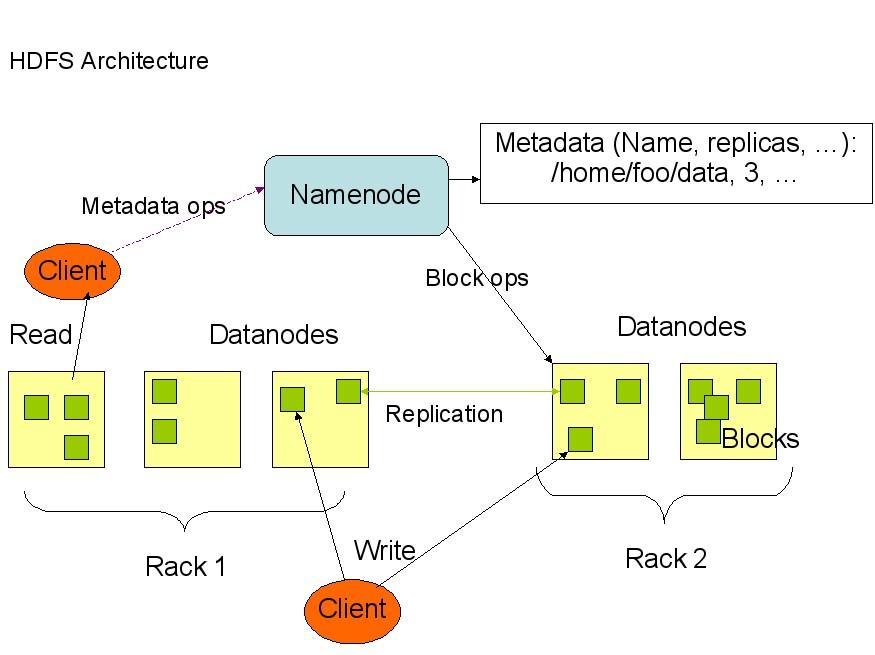
\includegraphics[scale=0.5]{photo/HDFS.jpg}
\caption{HDFS架构}
\end{figure} 


  第二个部分是MapReduce编程模型。它将并行计算性、容错性、负载均衡、数据分布方式等复杂的细节都封装在一个库里面,用户只要直接表述想要执行的简单运算即可。设计与实现Map/Reduce框架模型的突出优点是通过简单的接口来实现自动的并行化和大规模的分布式计算,并实现在大量的普通PC机上实施高性能计算。MapReduce将数据计算划分为两个步骤:分割计算(MaP)与合并统计(尺educe),这是其达到并行计算的主要工作方式。

  Hadoop技术已经在互联网领域得以广泛的应用。如Yahoo!使用Hadoop技术进行广告系统和Web搜索;Facebook使用Hadoop存储日志数据及之上的数据分析和机器学习;百度使用Hadoop进行搜索日志分析和网页数据挖掘工作以及淘宝使用Hadoop系统用来存储并处理电子商务的交易相关数据。


\section{一些解决方案}
  为了实现大量数据的实时性查询,主要有以下几种方案:
\subsection{RDBMS}
  典型的代表就是Mysql。它的优点有:模式固定,具有ACID性质和复杂的SQL查询处理引擎,能够保证数据的一致性和完整性。但另一方面,他也有许多难以避免的缺点,主要有:在上亿条记录里进行查询效率十分低下,无法进行简单的扩展。


  为了将Mysql满足海量数据查询的需要,就必须进行扩展为关系型数据库集群。当前的思路是随着数据量的增加,使得单点的结构变为主从型的分布,这样就能在从节点进行读操作,缓解了读操作时造成的IO压力。另外,如果数据库中的表数目较多,则可以将不同的表分开存储;如果某一个表太大,则可以把表分为不同的分区同样进行分布式存储。



\tikzstyle{block}=[rectangle,draw,fill=blue!20,text width=5em,
text centered,rounded corners,minimum height=4em]
\tikzstyle{line} = [draw, very thick, color=black!50]

\begin{tikzpicture}[node distance=3cm]
\node [block] (first) {单点db};
\node [block,right of=first] (second) {主从分布};
\node [block,right of=second] (third) {纵向切割};
\node [block,right of=third] (fourth) {横向切割};
\path [line] (first) -- (second);
\path [line] (second) -- (third);
\path [line] (third) -- (fourth);
\end{tikzpicture}

\subsection{Hive}
  Hive是建立在Hadoop上的数据仓库基础构架。它提供了一系列的工具,可以用来进行数据提取转化加载(ETL),这是一种可以存储、查询和分析存储在Hadoop中的大规模数据的机制。Hive定义了简单的类SQL查询语言,称为QL,它允许熟悉SQL的用户查询数据。同时,这个语言也允许熟悉MapReduce开发者的开发自定义的mapper和reducer 来处理内建的mapper和reducer 无法完成的复杂的分析工作。Hive没有专门的数据格式。Hive可以很好的工作在Thriff之上,控制分隔符,也允许用户指定数据格式。\cite{dataprocess}\cite{webfenxi}介绍了Hive的特点和日志分析的应用。


  下图是hive的架构: 


\begin{figure}[!ht]
\centering
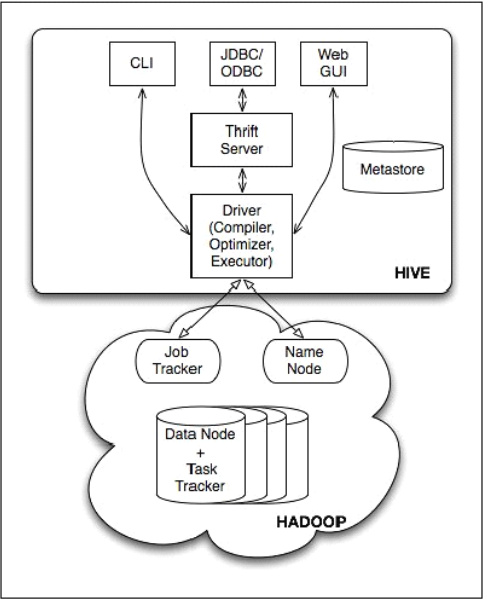
\includegraphics[scale=0.6]{photo/hive.PNG} 
\caption{Hive的架构图}
\end{figure} 


  Hive的用户接口包括CLI,Client和WUI。其中最常用的是CLI,Cli启动的时候,会同时启动一个Hive副本。Client是Hive的客户端,用户连接至HiveServer。在启动Client模式的时候,需要指出HiveServer所在节点,并且在该节点启动HiveServer。WUI是通过浏览器访问Hive。


  Hive将元数据存储在数据库中,如mysql、derby。Hive中的元数据包括表的名字,表的列和分区及其属性,表的属性(是否为外部表等),表的数据所在目录等。


  解释器、编译器、优化器完成HQL查询语句从词法分析、语法分析、编译、优化以及查询计划的生成。


生成的查询计划存储在HDFS中,并在随后有MapReduce调用执行。Hive的数据存储在HDFS中,大部分的查询由MapReduce完成。

\subsection{HBase}
  HBase 是一个高可靠性、高性能、面向列、可伸缩的分布式存储系统,利用HBase技术可在廉价PC Server上搭建起大规模结构化存储集群。


  HBase是Google Bigtable的开源实现,类似Google Bigtable利用GFS作为其文件存储系统,HBase利用Hadoop HDFS作为其文件存储系统;Google运行MapReduce来处理Bigtable中的海量数据,HBase同样利用Hadoop MapReduce来处理HBase中的海量数据;Google Bigtable利用 Chubby作为协同服务,HBase利用Zookeeper作为对应。

 
 HBase的服务器体系结构也是遵从简单的主从服务器架构,由Hregion服务器群和HBase Master主服务器构成。一般用表名+开始/结束主键来区分一个Hregion,一个Hregion会保存一个表里面某段连续的数据。一般一台机器上面运行一个Hregion服务器,而每一个区段Hregion只会被一个Hregion服务器维护。也就是说,HRegion是HBase中分布式存储和负载均衡的最小单元。但它并不是最小的存储单元。事实上,HRegion由一个或多个Store组成,每个store又由一个memstore和0至多个StoreFile组成。每个store保存一个column family。StoreFile以HFile的格式保存在HDFS上。


  下图是HBase的架构图: 
\clearpage

\begin{figure}[!ht]
\centering
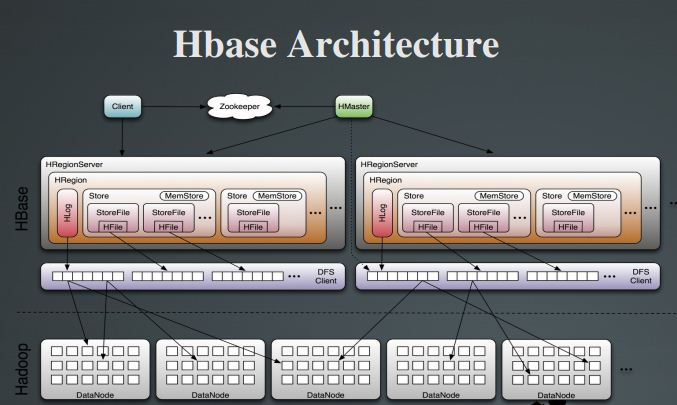
\includegraphics[scale=0.5]{photo/hbase.JPG}
\caption{HBase的架构图}
\end{figure}


  HBase的表由行和列组成,列划分为若干个列族。表中的row key是用来检索记录的主键,访问表中的行可以通过单个row key访问,也可以通过row key的range,还有就是全表扫描。行的一次读写是原子操作。


  Hbase表中的每一列都归属于某个列族,列族是表的chema的一部分(而列不是),必须在使用表之前定义,列名都以列族作为前缀。访问控制、磁盘和内存的使用统计都是在列族层面进行的。HBase中的表一般特点为大,甚至可以达到上百万行以至于上亿行;面向列,列族独立索引;稀疏,对于空的列,并不占用存储空间。下面是一个表的示例:

\begin{figure}[!ht]
\centering
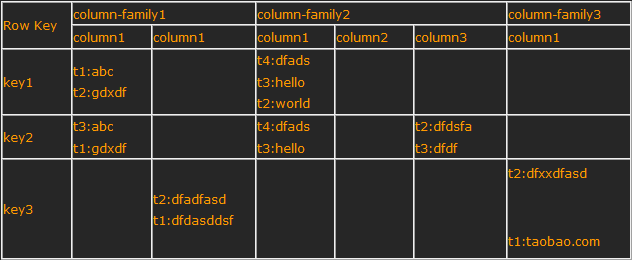
\includegraphics[]{photo/hbaseTable.PNG} 
\caption{HBase的表结构}
\end{figure} 

  从上面的表结构可以看出,Hbase的列不仅可以为空,亦可以动态进行增加,这就相对比较灵活。此外,Hbase的存储是自动分片的,少了人工操作的麻烦。它的缺点是没有一个功能强大的查询引擎,不支持复杂查询。

\subsection{MongoDB}
MongoDB是一个介于关系数据库和非关系数据库之间的产品,是非关系数据库当中功能最丰富,最像关系数据库的。他支持的数据结构非常松散,是类似json的bjson格式,因此可以存储比较复杂的数据类型。Mongo最大的特点是他支持的查询语言非常强大,其语法有点类似于面向对象的查询语言,几乎可以实现类似关系数据库单表查询的绝大部分功能,而且还支持对数据建立索引。\cite{MongoDBGuide}这本书比较详细的介绍了MongoDB的特性。

它的特点是高性能、易部署、易使用,存储数据非常方便。它扩展了关系型数据库的众多有用功能,如辅助索引、范围查询和排序,并且内置对MapReduce式聚合的支持,以及对地理空间索引的支持。它的数据模型对于开发者来说非常友好,配置选项也很轻松,并且有驱动程序和数据库shell提供的自然语言式放入API。MongoDB主要的功能特性有:
\begin{compactitem}
\item 面向集合存储,易存储对象类型的数据。
\item 模式自由。
\item 支持动态查询。
\item 支持完全索引,包含内部对象。
\item 支持查询。
\item 支持复制和故障恢复。
\item 使用高效的二进制数据存储,包括大型对象(如视频等)。
\item 自动处理碎片,以支持云计算层次的扩展性。
\item 支持RUBY,PYTHON,JAVA,C++,PHP等多种语言。
\item 文件存储格式为BSON(一种JSON的扩展)。
\item 可通过网络访问。
\end{compactitem}

\section{论文结构}
下面是这篇文章整体的布局情况。\\
\cvitem{0.132}{0.83}{第一章} {阐述选题的背景以及主要用到的几个开源软件的特点介绍。} \\
\cvitem{0.132}{0.83}{第二章} {阐述课题研究的方法;将hive与hbase的结合原理;实验的前提工作数据导入等等。} \\
\cvitem{0.132}{0.83}{第三章} {主要介绍了测试用到的几个实验,实验过程,实验结果及结论。} \\
\cvitem{0.132}{0.83}{第四章} {讨论了优化的方法如调整参数,使用索引,保证不倾斜;讨论了join算法。} \\
\cvitem{0.132}{0.83}{第五章} {介绍了HBase客户端编程的概念;针对一个条件查询编写了相应程序。}
